\documentclass[12pt]{article}
\usepackage[utf8]{inputenc}
\usepackage{sbc-template}

\usepackage{graphicx,url}
\usepackage{rotating}
\usepackage{dcolumn}
\usepackage{float}

\renewcommand{\figurename}{Figura}
\renewcommand{\tablename}{Tabela}
\renewcommand{\refname}{Referências}
     
\sloppy

\title{Problema 4: ``Batalha Naval"}

\author{Turma P04}


\address{MI - Projetos de Circuitos Digitais, Período 2015.1\\ Tutor: Marcos Paz\\
Curso de Engenharia de Computação \\ Universidade Estadual de Feira de Santana (UEFS)
}

\begin{document} 

\maketitle

\begin{resumo} 
O presente relatório descreve o processo de resolução do quarto problema do MI - Circuitos Digitais, da supracitada turma,no período de 2015.1, na Universidade Estadual de Feira de Santana. O problema propôs, dado o sucesso dos projetos pretéritos, que os estudantes desenvolvessem um protótipo do jogo Batalha Naval em \textit{FPGA}, tomando como base o  protótipo do controlador da matriz de \textit{LED}, sendo que a comunicação com este novo circuito deveria acontecer através de um computador pessoal utilizando o conceito de comunicação serial, tornando o projeto a ser desenvolvido, mais confiável em relação a transmissão de dados.
\end{resumo}

\section{Introdução}

Hoje em dia cresce, substancialmente, a ampla utilização de jogos no segmento lúdico de simulação 2D. Estes são utilizados em diversas áreas conhecidas, tendo uma mais elevada utilização na educação. Além do papel que os mesmos podem fornecer à educação, podem servir , também, única e exclusivamente como forma de entretenimento entre os mais jovens, bem como para o público mais adulto. Um exemplo destes jogos, é o famigerado Batalha Naval. Sendo lançado no Brasil no ano de 1988, o jogo batalha naval é um dos jogos de maiores sucessos entre o público mundial. Em sua forma mais rústica, dois adversários desenhavam em folhas de papel, navios posicionados em um mar imaginário quadriculado, formando uma grade. Ganhava aquele que descobrisse primeiro as coordenadas das embarcações do oponente. Todavia, no contexto atual, além de encontrar versões deste jogo de maneira similar aos seus primórdios, encontra-se, também, aplicativos para diversas arquiteturas que executam o mesmo processo, facilitando assim a sua disseminação entre as pessoas.

Além da existência, como visto, deste tipo de jogo na forma de aplicativos móveis, existe a possibilidade, também, de desenvolvê-lo utilizando circuitos digitais, visando a criação de um jogo lúdico de simulação 2D.  É de se notar, que para desenvolvê-lo, faz-se necessário utilizar um conceito muito importante na eletrônica digital, a saber, memória RAM. A criação deste tipo de jogo, traz diversas vantagens para o empreendedor que o desenvolve, justamente pelo fato do mercado de jogos está sempre em constante expansão. lembrando que hoje em dia, aplicações envolvendo a tecnologia digital tem ampla aceitação no mercado, o ser humano necessita de recursos tecnológicos, com forma também de pertença, e inclusão no mundo global tecnológico. 

Desta forma, observando a mudança atual do mercado, principalmente no que diz respeito a alta receptividade em relação a jogos eletrônicos, o grupo Inova Digital Bahia S.A  resolveu adaptar o projeto desenvolvido anteriormente, para que o mesmo funcionasse como uma espécie de jogo Batalha Naval, seguindo um modelo de simulação $2D$. Sendo que este novo protótipo deveria ser controlado remotamente, a partir de um computador pessoal, enviando os dados por meio de canal de comunicação serial. Neste jogo, dois modos estarão disponíveis, o modo de gravação e o modo de jogo propriamente dito, cada modo contendo suas especificações e características próprias, as quais serão descritas nas seções posteriores.

É importante lembrar, que para desenvolver este projeto, foram utilizados além dos recursos já conhecidos, fez-se uso também de Máquinas de estados, registrador de descolocamento, porta serial, protocolo de comunicação RS-232, conversores de níveis elétricos e, por último, mas não menos importante, Software para comunicação com Hardware.

\section{Fundamentação Teórica}

Na seção que segue, serão descritos os conceitos utilizados para resolução do problema proposto, frisando os conceitos que foram de fundamental importância para solucionar o mesmo, tendo contribuição de maneira direta ou indireta.

\subsection{Máquinas de Estados}
Em se tratando de Circuitos Digitais, diversos dispositivos têm uma ampla importância, dentre estes dispositivos temos os conhecidos contadores, os quais segundo\cite{tocci1997digital} são Máquinas de estados específicas. Floyd, por sua vez, vai mais adiante, e fala que Máquinas de estados ou circuito sequencial é um circuito que  consiste de uma seção de lógica combinacional e uma seção de memória (flip-flops)\cite{floyd2011digital}. Na figura~\ref{fig:diagrama-estados} podemos observar o circuito típico para uma máquina de estados. Vale acrescentar que a quantidade de estados que uma máquina pode interpretar é diretamente ligada a quantidade de Flip-Flop. A quantidade de estados pode ser obtido fazendo $2^{n}$, sendo n o número de Flip-flops.  

%TODO : Retirar esta figura
\begin{figure}[h]
\centering
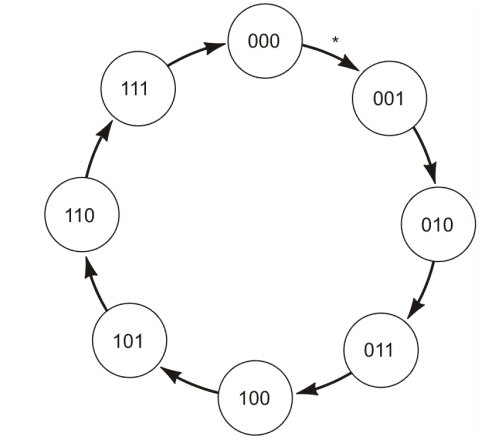
\includegraphics[width=.4\textwidth]{img/diagrama-estados.png}
\caption{Diagrama de estados de um contador de 3 bits\cite{floyd2011digital}}
\label{fig:diagrama}
\end{figure}

Existem basicamente, dois modelos de máquinas de estados, a saber, máquina Moore e máquina Mealy\cite{singh2006digital}. Na máquina Moore, a saída depende única e exclusivamente dos seus estados atuais, enquanto na máquina Mealy além de depender dos seus estados atuais, a saída depende, também, das variáveis de entrada naquele instante. Na figura~\ref{fig:diagrama-mealy}  podemos observar  o digrama de transição de estados para uma máquina Moore, já na figura~\ref{fig:diagrama-moore} temos o diagrama para uma máquina Mealy. É importante notarmos, através dos diagramas, a diferença referente a saída de cada máquina.   

\begin{figure}[h]
\centering
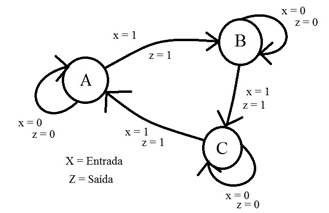
\includegraphics[width=.5\textwidth]{img/fig2MaquinaMealy.png}
\caption{Exemplo de diagrama de estados usando uma máquina Mealy}
\label{fig:diagrama-mealy}
\end{figure}

\begin{figure}[h]
\centering
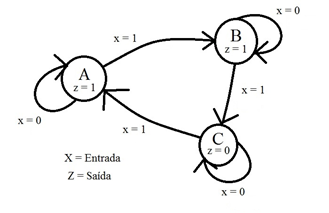
\includegraphics[width=.5\textwidth]{img/fig3MaquinaMoore.png}
\caption{Exemplo de diagrama de estados usando uma máquina Moore}
\label{fig:diagrama-moore}
\end{figure}

\subsection{Flip-Flop T}

Além dos Flip-Flops até o momento estudados, temos na literatura, outro Flip-Flop que é amplamente utilizado, qual seja, o Flip-flop T. Na figura~\ref{fig:fft} podemos analisar o bloco lógico e a tabela verdade para este Flip-Flop. Quando a entrada T estiver em estado alto, o Flip-Flop T, onde T significa \textit{toggle}, comutará quando o \textit{clock} for aplicado. Se a entrada T for baixa, o Flip-Flop mantém o valor do seu estado. Vale lembrar, que o Flip-Flop T pode ser obtido utilizando um Flip-Flop J-K, basta conectar as entradas J e K em nível lógico alto de maneira intermitente.  


%TODO: Colocar referncia da imagem https://pt.wikipedia.org/wiki/Flip-flop
\begin{figure}[h]
\centering
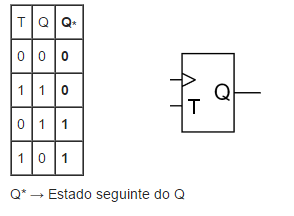
\includegraphics[width=.5\textwidth]{img/fig4Flip-Flopt.png}
\caption{Tabela Verdade do Flip Flop T}
\label{fig:fft}
\end{figure}

\subsection{Registrador de Deslocamento}

No universo dos circuitos digitais, principalmente no que diz respeito aos Flip-Flops, encontramos diversas aplicações. Uma, das várias aplicações é na forma de registrador de deslocamento, os quais são amplamente utilizados hoje em dia no desenvolvimento de circuitos robustos. Segundo \cite{floyd2011digital} os registradores de deslocamento consistem de arranjos de Flip-Flops e são importantes em aplicações que envolvem o armazenamento e a transferência de dados em sistemas digitais. É importante esclarecer, que o funcionamente do registrador de deslocamento é diferente de um contador comum, ou seja, ele não tem uma sequência específica de estados, apesar de em alguns casos poder ser utilizado como tal. Na figura~\ref{fig:rdeslocamento} podemos ver um circuito típico para um registrador de deslocamento de quatro bits com entrada e saída serial de dados.

\begin{figure}[h]
\centering
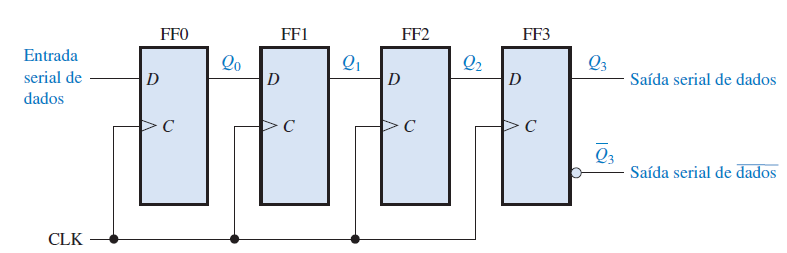
\includegraphics[width=.7\textwidth]{img/Fig5RegistradorDeslocamento.png}
\caption{Representação de um registrador de deslocamento de 4 bits \cite{floyd2011digital}}
\label{fig:rdeslocamento}
\end{figure}


São diversos, os tipos de registradores de deslocamento, na figura~\ref{fig:registradores} estes registradores de deslocamento são ilustrados de forma bem abstrata, porém compreensível. Dentre eles, um dos mais importantes é o registrador com entrada serial e saída paralela, o qual será abordado com mais detalhe na próxima sub-subseção.

\begin{figure}[h]
\centering
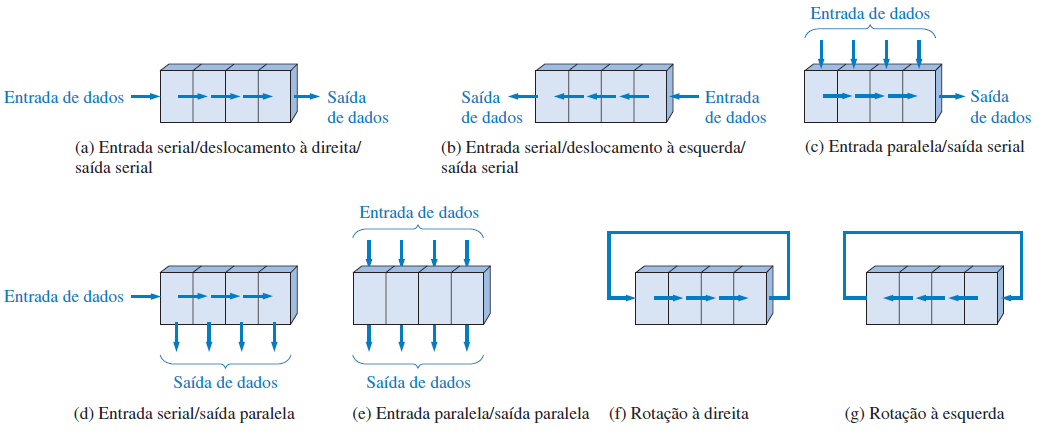
\includegraphics[width=.8\textwidth]{img/Fig6tipodeRegistrador.png}
\caption{Diferentes tipos de registradores, segundo \cite{floyd2011digital}}
\label{fig:registradores}
\end{figure}

\subsubsection{Registrador de deslocamento com entrada serial e saída paralela}

Como o próprio nome já designa, neste tipo de registrador, a entrada de dados se dá de forma serial, contudo, a saída não será serial e sim paralela. Desta forma, segundo \cite{floyd2011digital} uma vez armazenados os dados, cada bit aparece em sua linha de saída respectiva e todos os bits são disponibilizados simultaneamente, em vez de um bit de cada vez como no registrador com saída serial. Na figura~\ref{fig:registradorsp} podemos ver uma exemplificação para este circuito. Notem que neste tipo de registrador a saída de cada estágio está disponível após a aplicação do $clock$.

%TODO: Colocar a referência de FLOYD
\begin{figure}[h]
\centering
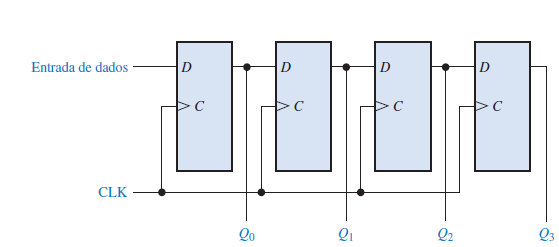
\includegraphics[width=.5\textwidth]{img/Fig7RegistradorSerialParalelo.png}
\caption{Registrador Serial-Paralelo}
\label{fig:registradorsp}
\end{figure}

\subsection{Comunicação Serial}
No contexto computacional, temos duas formas de comunicação principais, são elas: comunicação serial e comunicação paralela. cada uma com suas vantagens e desvantagens. Na comunicação paralela os bits são transferidos de maneira simultânea, conferindo para este tipo de comunicação a vantagem de rapidez e simplicidade de interface, contudo essa mesma vantagem acaba gerando algumas desvantagens, pois há um maior número de conexões, o que pode gerar ruído, perda de sincronismo, além de um custo maior. Já na comunicação serial os dados são transferidos  bit a bit, conferindo a vantagem de se ter menos fios, ou seja, baixo custo, além de ser capaz de transmitir dados em distâncias maiores. Contudo, nesta forma de comunicação, justamente por haver apenas um fio que transmite os dados, ela acaba sendo mais lenta, e com um grau de complexidade maior. Todavia, apesar das desvantagens da comunicação serial, a mesma se mostra mais robusta e mais viável a ser aplicada em sistemas onde a confiabilidade dos dados são importantes. Assim, esta subseção tratará especificamente deste tipo de comunicação. 

\subsubsection{Transmissão de Dados}
Antes de falarmos acerca de como ocorrer a transmissão de dados de forma serial, é importante lembrar que existe diversas interfaces que empregam este tipo de comunicação, entre as interfaces mais antigas estão as portas $DB9$ e $DB25$, as quais podem ser encontradas nos computadores mais antigos. Na figura~\ref{fig:db9db25} temos um exemplo para estas duas portas. Cada pino nestas portas tem uma determinada função, podendo variar de acordo com o seu tipo. Na  figura~\ref{fig:pinosdb9} podemos ver a função de cada pino para porta $DB9$.


%TODO: Colocar esta referência para imagem http://www.cerne-tec.com.br/Artigo_07_ComunicacaoSerial.pdf
\begin{figure}[h]
\centering
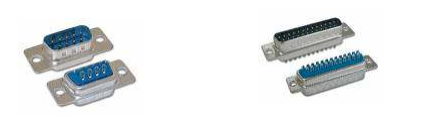
\includegraphics[width=.5\textwidth]{img/fig8DB9DB25.png}
\caption{Portas DB9 e DB25, interfaces seriais encontradas em computadores antigos.}
\label{fig:db9db25}
\end{figure}


%TODO: Colocar esta referência para imagem http://www.mecaweb.com.br/eletronica/content/e_serial
\begin{figure}[h]
\centering
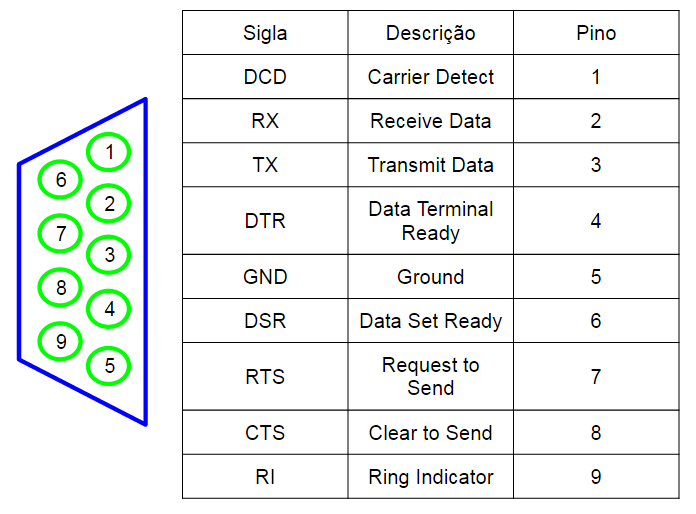
\includegraphics[width=.5\textwidth]{img/Fig9serial_pinos.png}
\caption{Funcionalidades dos pinos presentes na porta DB9.}
\label{fig:pinosdb9}
\end{figure}



Na maioria das aplicações, a comunicação serial acontece de forma assíncrona, onde geralmente se tem 11 bits sendo transferidos. Um desses bits é o \textit{start-bit}, o qual notifica um receptor que um novo dado serial está disponível, seguido pelos bits de dados, um bit opcional de paridade \textit{parity} e um ou mais bits de parada \textit{stop bits}\cite{porta-serial}. Percebam que o número de bits de paridade e de parada podem variar, dependendo apenas do padrão de transmissão escolhido pelo projetista. Na figura~\ref{fig:cserial} pode-se analisar esta forma de comunicação de maneira mais concreta. Vale acrescentar, que enquanto o bit de parada se manter em nível alto, os dados não serão transmitidos, e sim, apenas, quando ocorrer a mudança de estado do nível lógico alto para baixo, caracterizando assim, o bit de início, ou \textit{start bit}. 

%TODO: Colocar esta referência para imagem http://www.mecaweb.com.br/eletronica/content/e_serial

\begin{figure}[h]
\centering
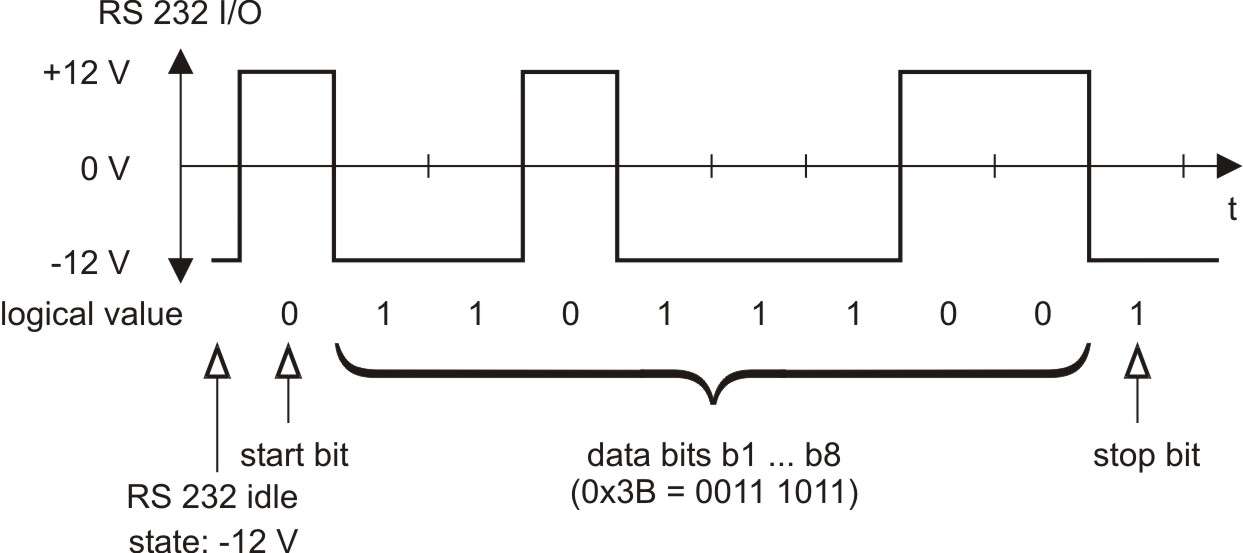
\includegraphics[width=.5\textwidth]{img/Fig10rs232.jpg}
\caption{Características de uma transferência de dados serial.}
\label{fig:cserial}
\end{figure}



Cada dispositivo que emprega a comunicação serial, tem uma determinada taxa de velocidade, sendo que para se referir a velocidade de transferência devemos usar o termo bps \textit{bits-per-second}, ou seja, bits por segundo. Em alguns equipamentos, costuma-se chamar esta taxa  como \textit{baud}. Desta forma, a expressão 9600 bps é equivalente a 9600 bauds.

\subsubsection{Padrão RS-232}
Segundo (http://www.c2o.pro.br/automacao/x834.html) RS-232 é um padrão definido pela \textit{EIA-Eletronic Industries Association} para os dispositivos usados para comunicação serial. Este padrão está disponível em três versões, quais sejam, (A, B e C). Cada um especifica uma faixa de voltagem para os níveis ligado e desligado. Por exemplo, na versão RS-232C, para representar  nível lógico alto utiliza-se as tensões de $-3V$ a $-12V$, enquanto para representar nível lógico baixo é utilizado tensão na faixa de $+3V$ e $+12V$. É importante notar que a representação de nível lógico alto e baixo nesse padrão, não utiliza o modelo convencional de tensão. Vale lembrar, ainda, que este padrão é utilizado marjoritariamente nas portas $DB9$ e $DB25$.  

\subsubsection{Conversor de nível MAX-232}
Os dispositivos eletrônicos utilizam níveis de tensão diferentes para identificar nível lógico baixo e nível lógico alto, dependendo apenas da tecnologia que está sendo empregada. Desta forma, quando se vai utilizar a porta serial do computador pessoal para se comunicar com algum dispositivo controlador, tem-se que analisar o padrão que o mesmo utiliza, pois a depender das especificações, será necessário fazer a conversão do nível. Por exemplo, vamos supor que queremos fazer uma comunicação entre o computador pessoal através da porta serial, com uma \textit{FPGA}. No entanto, a \textit{FPGA} utiliza a tecnologia \textit{TTL}, ou seja, de 0V a 0,8V representa nível lógico baixo e de $2V$ a $5V$ representa nível lógico alto. Percebe-se, assim, uma incompatibilidade entre o padrão RS-232 e o \textit{TTL}, desta forma é necessário fazer a conversão. Existe inúmeros dispositivos que tem a capacidade de fazer essa conversão, um deles é o MAX-232, o qual faz  a conversão entre os níveis utilizados pelo padrão RS-232 para TTL, e vice-versa. Na figura~\ref{fig:232} podemos ver uma configuração comum utilizando um conversor MAX-232. 

%TODO: colocar referencia na imagem https://www.sparkfun.com/images/tutorials/BeginningEmbedded/4-UART/UART1.jpg
\begin{figure}[h]
\centering
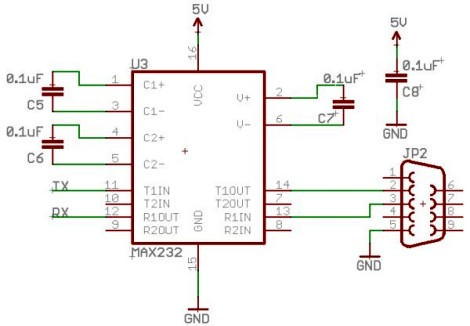
\includegraphics[width=.5\textwidth]{img/Fig11-microcontroller_uart_max232_circuit.jpg}
\caption{MAX-232: Conversor de RS-232 para TTL.}
\label{fig:232}
\end{figure}

\subsubsection{Software de comunicação}

O software é de fundamental importância para um bom funcionamento de qualquer hardware. Hoje em dia se pode fazer pequenos projetos, e programá-los utilizando alguma linguagem de programação especifica. Podendo ser um software que controle o circuito projeto totalmente, ou utilizado apenas para enviar dados para um circuito qualquer. Em muitos casos, para poder coletar os dados diretamente do usuário e enviá-los para o circuito, os mesmos precisam passar por um tratamento. Por exemplo, ao se elaborar um progrma para auxiliar no envio de dados pela porta serial do computador existe uma série de passos que deve ocorrer, como abrir a porta de comunicação, converter os dados inseridos pelo usuário em binário e, finalmente, enviá-los através da porta $DB9$.

\section{Metodologia}
Utilizando-se, mais uma vez, da base teórica fornecida pela metodologia $PBL$, os alunos componentes da turma T04 iniciaram as sessões destinadas a solução do problema com a leitura do mesmo em duas etapas, uma individual e outra coletiva. Tendo como objetivo a detecção inicial de dúvidas, fatos importantes relacionados ao problema e ideias de como solucnionar, o $brainstorm$ inicial ajudou a identificar as principais características do problema, fomentando ideias de como iniciar o desenvolvimento do mesmo.


Os membros da sessão, solucionando as questões um dos outros quando possível durante o processo, buscaram tomar decisões de projeto para formalização das obrigações, analisando fatores positivos e negativos das soluções propostas, optando pela solução que fosse mais simples e que estivesse de acordo com o problema, de acordo com a visão dos alunos do grupo. Com esse método deu-se início a construção da solução do problema 4 do MI - Circuitos Digitais, começando pela formalização e definição de padrões de projeto e de um diagrama que as mostrasse aplicadas ao circuito.

\subsection{Decisões de Projeto}

Antes de iniciar a implementação do projeto em si, foi necessário traçar o caminho a percorrer durante todo o processo de solução do problema. Essa metodologia foi adotada pelos membros da sessão após algumas decisões de projeto que não deram o resultado esperado nos problemas anteriores, causando incongruências entre os módulos projetados entre diferentes membros da turma. 


Dado o sucesso da abordagem no problema anterior, a turma decidiu continuar com a mesma linha de pensamento, ou seja, novamente dividir o problema em partes menores e atribuir a construção de cada parte a um subgrupo. Para aumentar a eficiência dessa abordagem, cada grupo deveria elaborar, também, um relatório que mostrasse o processo de construção e os conceitos utilizados na elaboração de cada uma das suas obrigações, além de entregar e descrever o bloco utilizando a ferramenta $EDA$ $Quartus II$. É importante afirmar que as tarefas não eram restritivas, sendo que cada grupo deveria, depois, estudar todos os outros circuítos tomando como base os relatórios elaborados pelos outros grupos. Para garantir que, quando fossem unidos, todos os blocos funcionassem, a turma elaborou um diagrama completo do problema, estabelecendo padrões para cada segmento.

\subsection{Elaboração do Diagrama}
Iniciado na primeira sessão do problema 4 e finalizado na terceira sessão do mesmo, o diagrama teve como objetivo fazer com que todos os alunos tivessem consciência plena do funcionamento do circuito, da entrada à saída, descrevendo as relações entre os blocos e sua respectiva função além da quantidade de entrada e a quantidade de saídas de cada um deles e padrões de nomenclatura. O diagrama descreve o que cada subgrupo deve fazer para que, quando combinadas, as frações do problema resultem em um circuito funcional e dentro da perspectiva do problema. 

O resultado desse processo de descrição em alto nível do projeto, pode ser conferido na figura~\ref{fig:diagrama}, a qual destaca também as tarefas de cada subgrupo. Por exemplo, o subgrupo vermelho é responsável pelo \textit{divisor de frequencia} e os \textit{contadores}.

\begin{figure}[h]
\centering
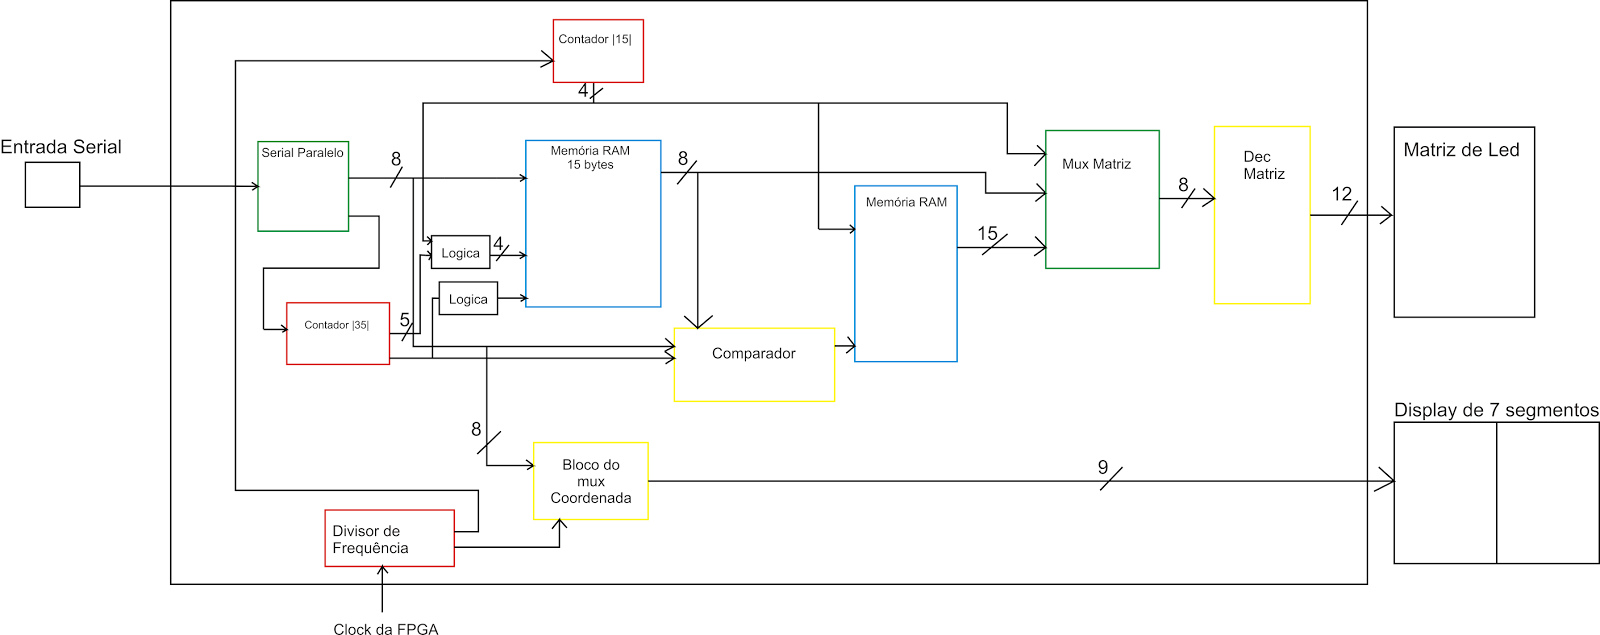
\includegraphics[width=1\textwidth]{img/diagrama.png}
\caption{Diagrama de blocos do Problema 4: Batalha Naval.}
\label{fig:diagrama}
\end{figure}


\subsection{Memórias RAM}

Como explicitado nas regras determinadas pela turma, o jogo será composto de 15 jogadas de preenchimento do tabuleiro mais 20 jogadas na qual o jogador tentará acertar o barco do oponente. A partir desse dado, é perceptível que precisam ser armazenados 15 posições diferentes, sendo cada uma correspondente a um pixel de um barco que foi inserido no tabuleiro, claro que ao nos referirmos a tabuleiro, estamos na verdade fazendo menção a matriz de $LEDs$. Utilizando a codificação de 8 $bits$ por coordenada, sendo 4 bits correspondentes a linha e outros 4 correspondentes a coluna. A partir dessas informações, chega-se a conclusão que a célula da memória $RAM$ deve ter 1 byte, e que a memória deve conter 15 dessas células.

Tendo em vista o mercado e a praticidade para uso em grandes escalas, a equipe resolveu construir uma memória com 16 células de 1 byte. Tal decisão foi tomada partindo dos princípios que o método de endereçamento da mesma não seria alterado, mas a 16ª célula ficaria ociosa. Porém, por ser uma potência de $2$, tal memória pode ser ligada em cascata de modo que um conjunto das mesmas possa, com facilidade, originar uma memória das capacidades comuns e requisitadas do mercado, como 512$MB$, 1$GB$, 4$GB$, entre outras.

Diferentemente do problema anterior, no Problema 4, o endereçador de memória foi integrado na mesma, objetivando uma maior congruência de projeto e uma visão mais limpa e ampla da totalidade do mesmo. Além dessa característica, como pode ser visto na figura~\ref{fig:ram15} a memória elaborada conta com 8 bits de entrada de dados a serem gravados ou lidos, um bit de $clock$, um bit de $clear$, um bit seletor $R/\overline{W}$ e 4 bits de endereçamento. Essa última característica segue o padrão crescente de 0 a 15, ou seja, o endereço 0 corresponde a primeira célula de memória, o 1 a segunda e assim por diante.


\begin{figure}[h]
\centering
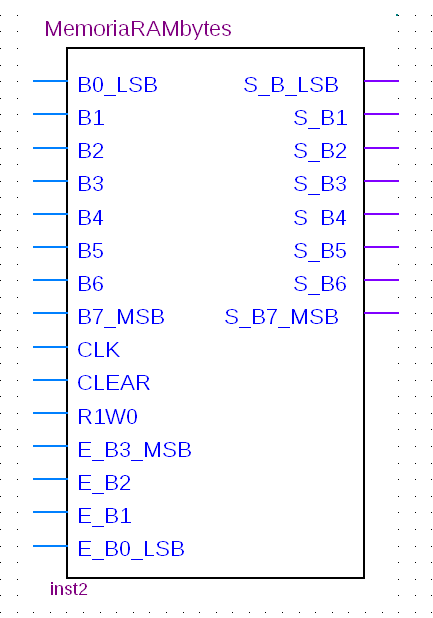
\includegraphics[width=.3\textwidth]{img/ram15bytes.png}
\caption{Bloco lógico da Memória Ram na EDA.}
\label{fig:ram15}
\end{figure}

\subsubsection{Célula de Memória}

Para elaborar o item anterior, fez-se necessário a elaboração de uma unidade básica de armazenamento, chamada de célula de memória. Para o problema 4, essa célula tem tamanho correspondente a 1 byte. Em suma, cada célula de memória do tipo demonstrado na figura ~\ref{fig:celulamemoria} funciona como uma miniatura da memória anteriormente citada, porém, se assim fêssemos pensar, ela só iria possuir um bit de endereçamento, uma vez que só existem duas possibilidades: ativada ou desativada.

\begin{figure}[h]
\centering
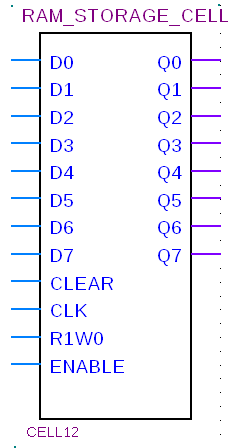
\includegraphics[width=.3\textwidth]{img/celulamemoria.png}
\caption{Bloco lógico da Célula da Memória Ram na EDA.}
\label{fig:celulamemoria}
\end{figure}

Buscando melhorar o desempenho da memória, em suas células foram implementados diferentes mecanismos, um deles permite que a mesma seja ligada, ou desligada completamente, já o outro faz com que a memória só seja gravada uma única vez, evitando possíveis dados duplicados e alteração indevida dos mesmos. O segundo mecanismo pode ser visto na figura~\ref{fig:ff1}. Esse mecanismo é uma máquina de estados de $Moore$ que está representada na figura~\ref{fig:fsm}. O outro mecanismo corresponde implementação da equação de excitação de um registrador do tipo T para as variáveis dadas. T deve mudar de estado quando sua saída $Q$ e sua entrada $I$ forem diferentes, e, além disso, a saída $Z$ do mecanismo anterior deve estar em nível lógico 1, ou seja: T= Z(Q$\oplus$I).

%A referencia da fsm no relatorio depois de compilado aparece mostrando que seria a imagem de numero 18, sendo que é a de número 16.


\begin{figure}[h]
\centering
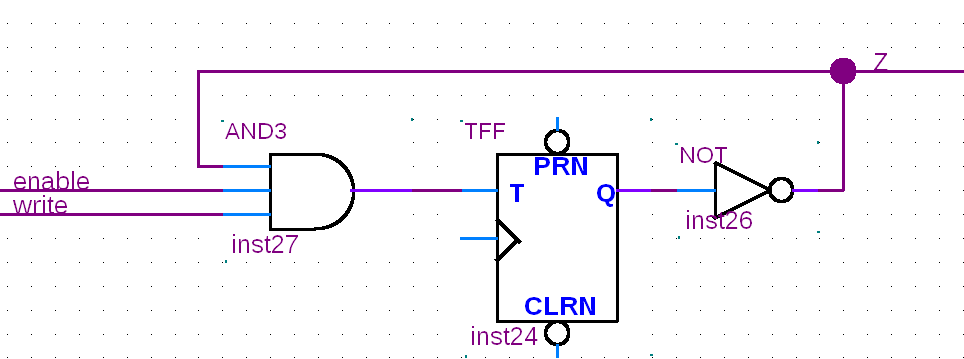
\includegraphics[width=.8\textwidth]{img/ff1.png}
\caption{Máquina de estados para máquina de uma única ação.}
\label{fig:ff1}
\end{figure}

\begin{figure}[h]
\centering
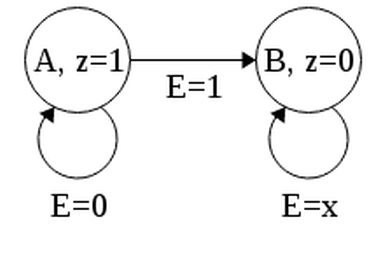
\includegraphics[width=.3\textwidth]{img/fsm.png}
\caption{Diagrama de estados para máquina de uma única ação.}
\label{fig:fsm}
\end{figure}


\subsubsection{Comunicação Serial}

Um, dos vários requisitos propostos pelo problema quatro, diz respeito a comunicação serial que deveria acontecer entre o computador pessoal e o Circuito Digital desenvolvido, onde esta, haveria de ser configurada no modo $start-stop assíncrono$, sendo que o frame de dados que seria utilizado nesse modo seria composto por 11 $bits$. Assim, é de se notar que a transferência de dados ocorreria utilizando alguma das portas seriais existentes em um computador pessoal. Desta forma, foi definido entre os membros do grupo que seria utilizada a porta serial $DB9$ para fazer essa comunicação no projeto que estava sendo desenvolvido, ou seja, seria utilizado o padrão $RS-232$ de comunicação de dados.

Depois de definir que seria utilizado a porta $DB9$, era necessário criar um circuito que fosse capaz de identificar quando essa transferência estivesse acontecendo, ou seja, um circuito que fosse capaz de reconhecer quando o computador estava enviando um $frame$ de dados para $FPGA$. Este circuito deveria ser capaz, ainda, de transformar os dados que estavam sendo transferidos na forma serial, para o formato paralelo, tornando assim possível a leitura correta dos dados, possibilitando o seu uso em outra parte do circuito. A figura~\ref{fig:aa2} mostra os blocos lógicos para este circuito. Nesta figura, podemos observar três blocos de grande importância, a saber, o bloco $AtivaRecepcao$, outro bloco chamado $Contador$, e mais um chamado  de $RegistraDados$. O $AtivaRecepcao$ é responsável, como o próprio nome dele já deixa explicito, por ativar a recepção do $frame$ de dados advindos da porta serial do computador pessoal. Quando o $start-bit$ é detectado, a entrada $Enable$ deste bloco muda para nível lógico alto, ativando assim o bloco $RegistraDados$, o qual inicia de fato a leitura do $frame$ de dados enviados. Percebam que neste mesmo bloco temos uma entrada chamada $DadosLidos$, esta entrada é responsável por levar o $Enable$ novamente para nível baixo, tornando possível uma nova leitura. Sendo que a entrada é correspondente ao $stop-bit$, ou seja, o último bit do $frame$ de dados, indicando que aqueles determinados dados foram lidos com sucesso. Pelo fato da simplicidade do circuito interno, o mesmo não será exibido. 


\begin{figure}[h]
\centering
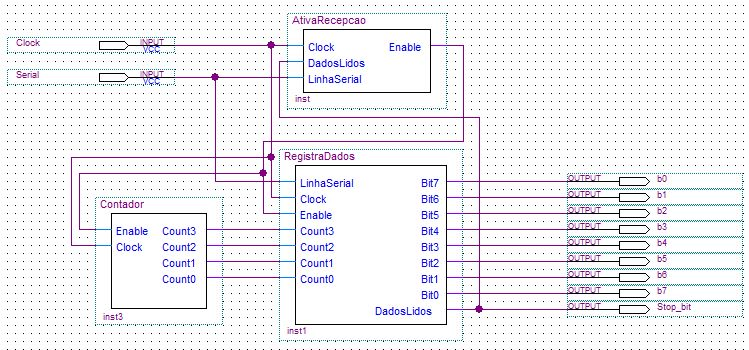
\includegraphics[width=1\textwidth]{img/aa2.jpg}
\caption{Circuito Conversor Serial-Paralelo.}
\label{fig:aa2}
\end{figure}

\begin{figure}[h]
\centering
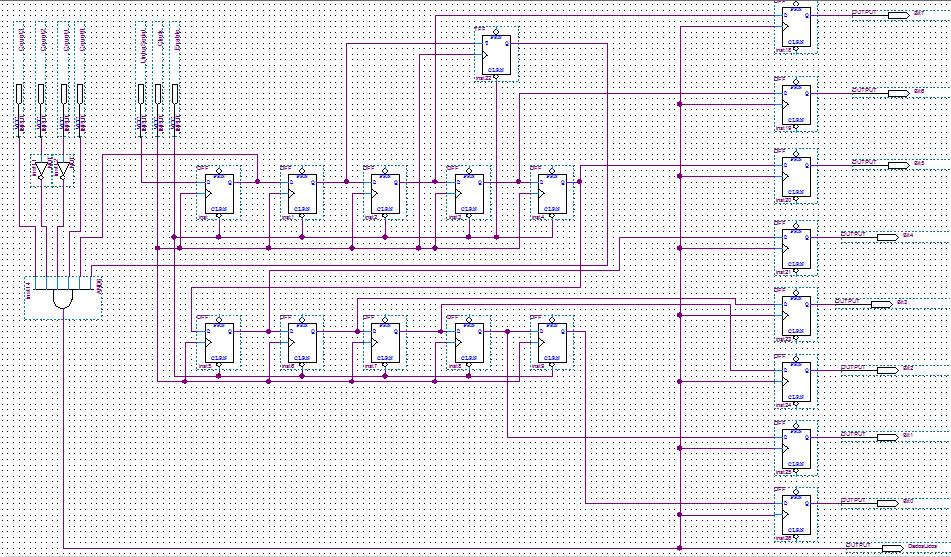
\includegraphics[width=1\textwidth]{img/aa1.jpg}
\caption{Circuito RegistraDados.}
\label{fig:fsm}
\end{figure}


Já o bloco Contador, tem uma função por demasiada simples, ele é ativado quando se inicia a leitura de um $frame$ de dados. Ele é um contador de módulo 11, ou seja, é capaz de gerar 11 estados distintos. Ele é utilizado para ativar a saída dos dados lidos serialmente, ou seja, depois que os $bits$ vindos do canal de comunicação serial forem lidos e convertidos para o formato paralelo, o contador estará no seu 11º estado, qual seja, 1010, esse mesmo valor é decodificado, ativando assim a saída de dados do registrador paralelo, pois esse valor decodificado gerará um nível lógico alto, onde esse valor alto é a entrada do $clock$ do registrador paralelo presente no bloco $RegistraDados$. Essa ideia tornar-se-á mais clara depois que o circuito interno do bloco $RegistraDados$ for observado. É importante salientar, também, que o circuito interno do contador não será mostrado, devido, é claro, a sua simplicidade de implementação.


%TODO trocar o nome ANEXO, Para uma referencia a figura dinamica. está na segunda linha do paragrafo.

O bloco $RegistraDados$, dentre, os blocos descritos, é o mais importante, pois ele é o responsável, por, de fato, armazenar e transformar os $bits$ do formato serial para paralelo. O circuito interno para este bloco pode ser observado no ANEXO 1.  O funcionamento deste bloco é bem simples. Depois de ativado, inicia-se a leitura e conversão dos dados para o formato paralelo a cada pulso do $clock$, sendo que o registrador de entrada de dados, está conectado, também, a outro registrador de saída de dados, onde cada $Flip-Flop$ de acordo com seu valor posicional estão conectados entre si. Observem que os dados que estão no registrador de saída de dados, só estarão disponíveis, realmente, quando o valor do contador estiver em 10, evidenciando assim, que todos os $bits$ foram lidos de forma correta, podendo desta forma, serem disponibilizados para outra aplicação fazer uso.  É importante salientar, que depois que este conjunto de dados forem lidos, tanto o bloco $AtivaRecepcao$, quanto o bloco $Contador$, serão reiniciados, podendo, então, serem utilizados na recepção de outro conjunto de $bits$.

Vale asseverar, que os bits advindos da porta serial estão sendo transferidos a uma taxa de 9600 $bits$ por segundo, ou 9,6$Kbs$. Isto foi definido no $software$ que fora desenvolvido tendo como objetivo justamente fazer esta interface entre o usuário e o circuito projetado. Lembrando que, para ajudar as realizar as tarefas correspondentes ao manuseio de permissões e envio de dados, foi utilizada a biblioteca $RS232$, construída em linguagem C e disponível e documentada em $http://www.teuniz.net/RS-232/$.

Quando se fala em comunicação serial, o sincronismo utilizado para recepção dos dados, deve ser observado de forma minuciosa, visando a leitura correta dos dados que estão no $frame$.  Desta forma, tentando resolver o problema do sincronismo no projeto desenvolvido foi utilizado o seguinte pensamento: como a frequência do $clock$ da $FPGA$ é de 32,768 $MHZ$ e a taxa de $bits$ por segundo utilizada na programação é de 9600 $bps$, fazendo 32768000/x = 9600, teremos X valendo aproximadamente 3413, ou seja, usando um contador de módulo 17 para alternar um $Flip-Flop T$ e obter uma frequência 34 vezes menor, sendo que em seguida foi necessário inserir um contador de módulo 100 para dividir a frequência por 200.Tendo assim, um pulso de $clock$ a cada bit enviado.

\subsection{Unificação dos blocos em um projeto}

Diferentemente do problema anterior, no problema 4 as tarefas foram dadas como prioridades a um subgrupo, ou seja, um grupo se encarregaria da montagem de um item, enquanto outro grupo se dedicava a outro módulo do problema. Apesar dessa divisão, ao final, todos os grupos deveriam intercambiar o conhecimento adquirido no processo com os demais participantes. Mesmo estando responsáveis por uma tarefa específica ao grupo, isto não tirava de ninguém a responsabilidade de montar por si só o circuito novamente, em busca de compreender por inteiro o funcionamento do mesmo.

Ao receber os blocos, não foi difícil montá-los em um único projeto, uma vez que, semelhante ao problema anterior, teve-se ao lado, um diagrama com todas as conexões e padrões de cada unidade lógica ali presente, e, além disso, todas elas já estavam devidamente testadas, eliminando chances de haverem problemas relacionados ao mal funcionamento de alguma das unidades. Feita a montagem, a mesma foi disponibilizada para o grupO, visando a análise e verificação de erros. Ao término da montagem nenhum erro foi verificado.

\subsection{Refatoração do circuito na protoboard}

Para que fosse viável utilizar a transmissão serial de dados, o circuito físico precisava ser modificado, adicionando desta forma um conversor de nível de tensão, alguns capacitores e um cabo de transmissão serial. Além disso, muitos dos componentes do problema anterior puderam ser retirados, muitos deles relacionados a entrada de dados, tais como o DIP Switch e resistores de $pull-down$. Um dos itens adicionados a $protoboard$ foi o MAX-232, um circuito que converte a tensão vinda da porta $DB9$ do computador para a tensão na faixa $TTL$. Para funcionar corretamente, o mesmo foi adicionado ao circuito seguindo as instruções da figura~\ref{fig:max232}.


%TODO: Colocar referencia dessa imagem https://www.sparkfun.com/images/tutorials/BeginningEmbedded/4-UART/UART1.jpg
\begin{figure}[h]
\centering
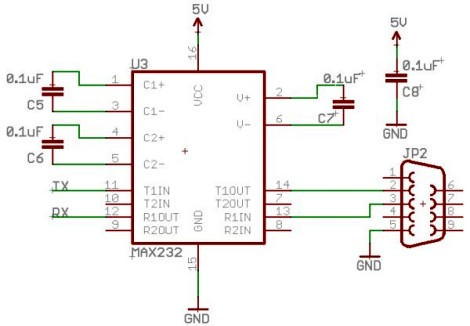
\includegraphics[width=.8\textwidth]{img/232.jpg}
\caption{Circuito do MAX-232.}
\label{fig:max232}
\end{figure}

Para o cabo de comunicação, foi utilizado um cabo antigo presente no laboratório e uma porta $DB9$ fêmea. Tendo este cabo em mãos, bem como a porta fêmea, foi necessário fazer a soldagem do mesmo para que ele pudesse ser utilizado na transmissão de dados. No $DB9$ foram soldados fios nas entradas $TX$, $RX$ e $GND$, mesmo sabendo que apenas a porta $TX$ seria usada, uma vez que os dados seguiriam uma via única do computador para o circuito.

\section{Discussões e resultados}

Nesta seção serão abordados os principais resultados obtidos, os testes realizados e, além disso, serão abordados alguns detalhes que dizem respeito ao circuito lógico.

\subsection{Testes lógicos no ambiente Quartus II}

Passados como tarefas para os subgrupos, os testes lógicos foram realizados bloco-a-bloco, tentando diminuir ao máximo a chance de qualquer erro de implementação de lógica. Para os testes da memória RAM de 15 bytes e do conversor serial-paralelo, dado o fato que esses são os únicos itens que o grupo não trabalhou ou conhece na escala exigida pelo problema.

\subsubsection{Testes da Memória RAM}

Inicialmente, foi feito um conjunto de testes básicos para verificar se a memória estava sendo capaz de distinguir os momentos de gravação/leitura, e gravando apenas um dado por célula. Para isso, foi fixado uma célula(vide figura~\ref{fig:ramtest}, referente ao endereço $EB0=0, EB1=0, EB2=0, EB3=0$). Avaliando os resultados, percebe-se uma constante nas saídas $0,1,2,3,4,5,6,7$ que equivalem aos primeiros valores enviados no modo de gravação, apontando o sucesso do teste.

\begin{figure}[h]
\centering
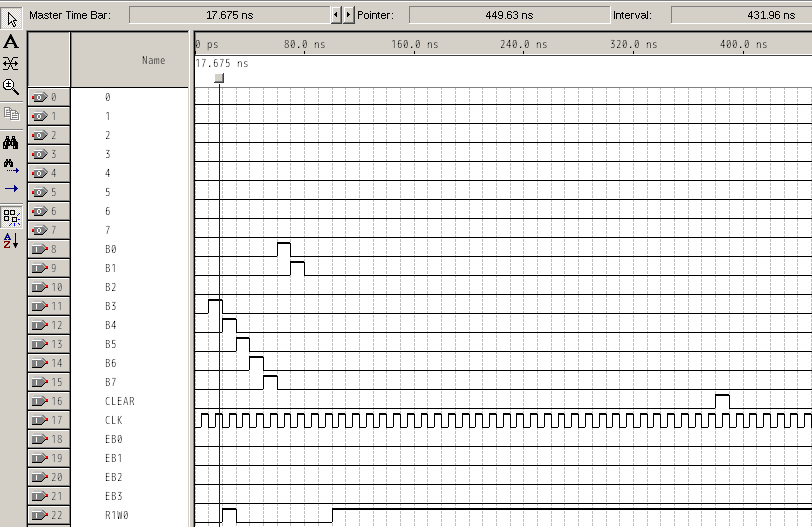
\includegraphics[width=1\textwidth]{img/testram1.png}
\caption{Teste de persistência e modo de operação}
\label{fig:ramtest}
\end{figure}

Prosseguindo os testes, o teste anterior foi repetido em uma escala de variação maior e utilizando-se todos os endereços disponíveis da memória $RAM$. O esperado é que a saída equivalesse ao primeiro valor de entrada em cada uma das células, e para cada período de $clock$ entre 1 e 15, as entradas deveriam equivaler as saídas quando a memória estivesse em modo leitura. Ou seja, estando em $loop$ de entradas constantes, quando a memória estiver no modo de leitura, esta, vai "imitar" as 16 primeiras sequências de entrada, como demonstrado com sucesso no teste descrito na figura~\ref{fig:ramtest2}.

\begin{figure}[h]
\centering
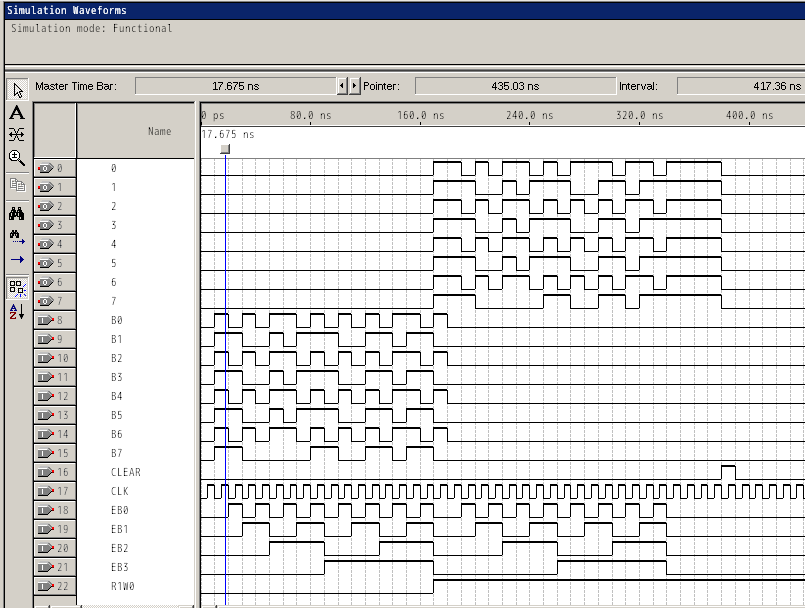
\includegraphics[width=1\textwidth]{img/testram2.png}
\caption{Teste de persistência e modo de operação}
\label{fig:ramtest2}
\end{figure}

\subsection{Funcionamento do Circuito}
Segundo os requisitos do Problema 4, o usuário deve entrar com coordenadas em um software que se encarregará de direcionar os dados para o circuito, no qual o tratamento de dados será feito. A partir desses dados, existem dois momentos:

\begin{itemize}
\item Modo Gravação: O usuário insere 15 coordenadas nas quais deseja que fiquem seus barcos, inicialmente todos os $pixels$ da matriz estão apagados.
\item Modo Jogo: O usuário tenta acertar os $pixels$ que representam barcos, caso acerte, o pixel acende. O número máximo de tentativas é de 20, e caso não consiga encontrar todos os barcos, o jogo é encerrado.
\end{itemize}


\subsection{Testes práticos}
Antes de realizar os testes do circuito na $Protoboard$, fazia-se necessário fazer a demarcação dos pinos adicionais na ferramenta $Quartus II$ e  gravar o circuito lógico do mesmo na $FPGA$ disponível no laboratório. Dada significante diminuição de uso dos pinos do problema 3 para o problema 4, não foi necessária a demarcação  de outros pinos, reaproveitando alguns deles que foram utilizados no problema 3, para ser aplicados, agora, no problema 4. Ligados os novos componentes, o circuito foi ligado e a gravação foi feita.

Dispondo-se de todas as ferramentas necessárias, o teste foi realizado introduzindo-se todas as coordenadas possíveis via $software$, e em um primeiro momento foi constatado que nada acontecia, mesmo seguindo à risca todas as orientações definidas pelo grupo. Suspeitando o não funcionamento da comunicação serial, dada a inexperiência da equipe com esse tipo de comunicação, foram anexados a $Protoboard$ um conjunto de $LED's$ para analisar se os dados estavam sendo transmitidos corretamente. Para ser capaz de tal tarefa, as saídas do bloco conversor serial/paralelo foram diretamente ligados as saídas que representavam os $LED's$, com isso pretendia verificar se o conversor serial-paralelo estava funcionando como o esperado. Dessa forma, para qualquer coordenada válida inserida, eles deveriam acender, representando assim, os bits enviados.


Desta forma, observando a saída emitida pelos $LEDs$, foi constatado que os dados não estavam sendo transmitidos ou recebidos corretamente, eliminando a variável de transmissão como fator de causa do problema, uma vez que ela é provinda do computador e o funcionamento é garantido, restou para a recepção dos dados. Analisando cuidadosamente a situação, o grupo entendeu que o $clock$ presente no circuito lógico conversor não estava sendo capaz de recepcionar corretamente todos os dados, ou seja, não havia uma borda de subida do mesmo entre cada período do $frame$ de dados recepcionado. Buscando solucionar o erro, a equipe realizou cálculos tendo como referência o $clock$ da $FPGA$(32.768$MHz$) e a taxa de transferência escolhida(9600$bps$), implementou-se um contador de módulo 3400 ao associar os contadores já existentes. Tal contador foi utilizado como um divisor de frequência para o $clock$ da $FPGA$, chegando-se a uma frequência próxima a requerida pela transmissão. Ao realizar novamente os testes, os $LEDs$ acenderam da forma esperada, porém, ao repetir o processo algumas vezes, detectou-se erros nos bits transmitidos. Tais erros são proveniente da influência de ruídos e de campos elétricos presentes no ambiente de prototipagem. Para evitar esses erros, poderia ser feito uma verificação de paridade, porém a paridade oferecida pelo esquema de transmissão utilizado é muito simples e não eficiente, ou seja, não resolve totalmente os problemas. Por essa razão, o grupo optou por não utilizá-la.

Desta forma, não se sabe ao certo como solucionar este problema, pois foram realizadas várias verificações e não se obteve êxito, mesmo depois de modificar a taxa de leitura dos dados da comunicação serial. Houve a diminuição de erros, mas mesmo assim continua dando erro em algumas coordenadas que são inseridas, ou seja, a recepção de dados realiza a leitura correta em apenas um momento, depois as leituras sucessivas são incorretas. 


%TODO: Colocar figura referente ao projeto final, nao esuqeça de tirar o nome figura que está em maiusculo.
\subsection{Circuito Final}
O circuito final do projeto desenvolvido pode ser visualizado  na FIGURA TAL, percebam que ele ainda está com os $LEDs$, que foram utilizados nos teste práticos, visando identificar os erros de sincronização. É importante perceber, também, que além dos 8 $LEDs$ que representam a coordenda de alguma posição na matriz, temos mais um $LED$ que é responsável por verificar se os dados estão sendo enviados, ou seja, quando algum dado for enviado ele acenderá momentaneamente. Isto foi feito para verificar se a configuração de envio de dados do circuito final estava funcionando.

\section{Conclusão}

Observando os requisitos para o desenvolvimento deste circuito digital, é notável que nem todas as funcionalidades foram alcançadas. A configuração $start-stop$ assíncrona não foi obtida em sua totalidade, pois ao fazermos os testes físicos utilizando $LEDs$ para visualizar os $bits$ que estavam sendo lidos, em certos momentos as coordenadas corretas eram visualizadas, contudo, ao enviar outras coordenadas o mesmo não acontecia. Acredita-se que isso pode ser devido ao problema de sincronização da comunicação depois de um certo tempo de transmissão. Mesmo depois de realizar diversos testes no circuito projetado, não se obteve êxito, tornando, a partir disso, inviável a utilização do modo jogo a partir da comunicação serial. Persistiu-se com os testes físicos, mesmo fazendo modificações no $clock$ responsável por fazer a leitura do $frame$ de dados, mas nem assim foi possível obter um valor exato para leitura dos dados advindos do computador pessoal.


Afora este problema relatado acima, todas as outras funcionalidades estão funcionando conforme o solicitado, ou seja, a lógica de resolução do problema está correta. Isto se torna mais concreto devido ao sucesso fatídico alcançado através dos testes realizados. Tendo sido revisado e simplificado várias vezes utilizando métodos específicos para a tarefa até chegar ao sistema mais simples, funcional e profícuo. De maneira semelhante aos problemas anteriores, o circuito final deste problema manteve uma boa ergonomia, inclusive foi adicionando um botão na $protoboard$, tendo como objetivo limpar a memória $Ram$, tornando possível a inicialização de outra partida do jogo batalha naval. 

Vale acrescentar, que os conteúdos estudados para resolução do problema, os quais de uma certa maneira gerou conhecimento, tanto em grupo quanto individualmente, são de fundamental importância na área da eletrônica, principalmente em relação a comunicação serial de dados, a qual é amplamente utilizada hoje em dia. Não se pode esquecer, é claro, das máquinas de estados, as quais são utilizadas em muitas aplicações. Sendo assim, estes conteúdos, e outros mais, irão contribuir de forma significativa para o bom desenvolvimento profissional de cada integrante do grupo e também facilitarão o entendimento de conteúdo futuros dentro do curso, haja vista que eles têm uma conexão muito forte com outros conteúdos do mundo da eletrônica, os quais ainda serão estudados.


\section{Referências}

Nessa seção constam os trabalhos utilizados como base teórica que foram necessários para chegar a solução descrita nesse relatório.


\bibliographystyle{sbc}
\bibliography{sbc-template}

\end{document}
